\begin{frame}
\frametitle{Line from Point and Direction}
\begin{columns}
\column{0.3\textwidth}
\psset{xunit=1cm, yunit=1cm}
\begin{pspicture}(-0.2,-0.2)(3.5,2)
\tiny
\fcFullDot{0}{0}
\rput[tl](0,-0.1){$O$}
\psline(0, 1.7)(3.5,0.3)
\fcFullDot{0.5}{1.5}
\rput[bl](0.5, 1.5){$P_0$}
\uncover<4->{
\psline[arrows=->, linecolor=red](0.5,1.5)(2.5,0.7)
}
\psline[arrows=->, linecolor=blue](1,1.3)(2, 0.9)
\rput[b](1.5,1.2) {$\fcv u$}
\rput[l](3.5,0.3){$L$}

\uncover<2->{\psline[arrows=->](0,0)(0.5,1.5)
\rput[l](0.25, 0.75){$~~\fcv r_0$}
}
\uncover<3->{%
\psline[arrows=->](0,0)(2.5, 0.7)
\rput[b](2.5, 0.75){$P$}
\rput[t](1.25, 0.2){$\fcv r$}
}
\end{pspicture}

\column{0.7\textwidth}
\begin{itemize}
\item Suppose we have line $L$ that passes through point $P_0$ and has non-zero direction $\textbf{u}$.
\item<2-> Denote by $\fcv r_0=\fcv{OP}_0$ the position vector of $P_0$.
\item<3->$P$ with position vector $\textbf{r}$ is on $L$ $\Leftrightarrow$ 
\item<4->$\textbf{P}_0\textbf{P}$ has the same direction as $\textbf{u}$ $\Leftrightarrow$
\item<5-> $\textbf{P}_0\textbf{P}$ is a scalar multiple of $\textbf{u}$ $\Leftrightarrow$
\item<6-> $\textbf{r}-\textbf{r}_0 = t\textbf{u}$  for some real number $t$.
\end{itemize}
\end{columns}
\uncover<7->{
\begin{definition}
The equation 
\[
\fcv{r} = \fcv{r}_0+t\fcv{u}
\]
is called a parametric vectorial equation of the the line $L$.
\end{definition}
}
\end{frame}

\begin{frame}
\frametitle{Line from Point and Direction}
\begin{columns}
  \column{6cm}
\begin{itemize}
 \item Point $P_0(x_0,y_0,z_0)$, $\textbf{r}_0=\langle x_0,y_0,z_0\rangle$;
\item Direction $\textbf{u}=\langle u_1,u_2,u_3\rangle$.
\end{itemize}
  \column{5cm}
 $L$: line with direction $\textbf{u}$, \\passing through $P_0$
\end{columns}

\begin{columns}
  \column{6cm}
    \uncover<2->{$P$ with position vector $\textbf{r}$ is on $L$ $\leftrightarrow$ \\ }
    \uncover<3->{\medskip $\textbf{r} = \textbf{r}_0+t\textbf{u}$ $\leftrightarrow$\\}
    \uncover<4->{\medskip $\langle x,y,z\rangle = \langle x_0,y_0,z_0\rangle + t\langle u_1,u_2,u_3\rangle$ $\leftrightarrow$\\}
    \uncover<5->{\medskip \textcolor[rgb]{0.98,0.00,0.00}{Parametric scalar equations}:\\
    $\boxed{\left\{ \begin{array}{ll}
           x & = x_0 + t u_1 \\
	   y & = y_0 + t u_2 \\
           z & = z_0 + t u_3
          \end{array}
\right.}$  \\ for some real parameter $t$ }

  \column{6.5cm}
    \begin{figure}
        \psfrag{O}{$O$}
        \psfrag{x}{$x$}
        \psfrag{y}{$y$}
        \psfrag{z}{$z$}
        \psfrag{L}{$L$}
        \psfrag{P}{$P(x,y,z)$}
        \psfrag{P0}{$P_0(x_0,y_0,z_0)$}
        \psfrag{r}{$\textbf{r}$}
        \psfrag{u}{$\textbf{u}=\langle u_1,u_2,u_3\rangle$}
        \psfrag{r0}{$\textbf{r}_0$}
        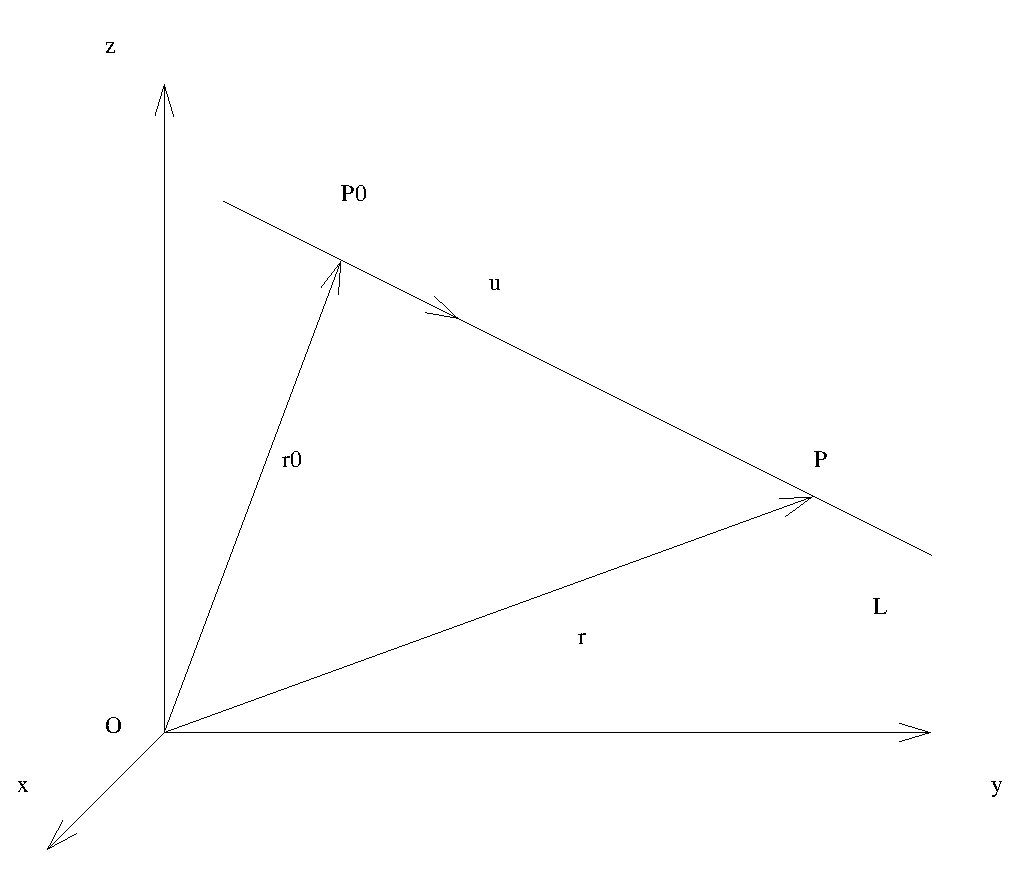
\includegraphics[height=2in]{../../modules/vectors/pictures/ok-line_point_direction_scalar.eps}
    \end{figure}
\end{columns}
\end{frame}

\begin{frame}
\uncover<1->{ $$\left\{ \begin{array}{ll}
           x & = x_0 + t u_1 \\
	   y & = y_0 + t u_2 \\
           z & = z_0 + t u_3
          \end{array}
\right. \Longrightarrow \boxed{\frac{x-x_0}{u_1} = \frac{y-y_0}{u_2} = \frac{z-z_0}{u_3}} \text{ \textcolor[rgb]{0.98,0.00,0.00}{Symmetric equations}}$$}

\uncover<2->{Caution! If $u_2=0$ (for example), then:
%
$$\frac{x-x_0}{u_1} = \frac{z-z_0}{u_3} \quad  \text{ and } \quad y=y_0 $$}

\uncover<3->{Example: Line with direction $\textbf{u} = \langle 4,5,6\rangle$ through $P_0(1,2,3)$:}
\begin{itemize}
 \item<4-> Parametric vectorial equation:
%
$$\textbf{r} = \langle 1,2,3\rangle + t \langle 4,5,6\rangle \leftrightarrow
\textbf{r} = \langle 1+4t, 2+5t, 3+6t\rangle$$
%
\item<5-> Parametric scalar equations:
%
$$\left\{ \begin{array}{ll}
           x & = 1 + 4t \\
	   y & = 2+5t \\
           z & = 3+6t
          \end{array}
\right. , \quad t \text{ real number.}$$
%
\item<6-> Symmetric equations:
%
$$\frac{x-1}{4} = \frac{y-2}{5} = \frac{z-3}{6}\; .$$
\end{itemize}

\end{frame}